% SPDX-FileCopyrightText: © 2024 Sebastian Davids <sdavids@gmx.de>
% SPDX-License-Identifier: Apache-2.0

\documentclass[a4paper]{germanarticle}

\usepackage{blindtext}
\usepackage{amsmath}
\usepackage{pgfplots}

\usepackage{color}
\definecolor{sc_keyword}{RGB}{0, 51, 179}
\definecolor{sc_string}{RGB}{6, 125, 23}

\usepackage{listings}
\lstset{
  basicstyle=\sffamily,
  keywordstyle=\color{sc_keyword},
  stringstyle=\color{sc_string},
  numbers=left,
  numberstyle=\tiny,
  frame=tb,
  tabsize=2,
  columns=fixed,
  showstringspaces=false,
  keepspaces=true,
}

\pagestyle{empty}

\begin{document}

\Huge\LaTeX\normalsize

\blinddocument

\section{Source Code}
  \begin{verbatim}
void main() {
  println("Hello world!");
}
  \end{verbatim}
  \begin{lstlisting}[language=Java]
void main() {
  println("Hello world!" + 1);
}
  \end{lstlisting}

\section{Equation}
  \begin{equation*}
    \sqrt{x^2+1}
  \end{equation*}

\section{Plot}
  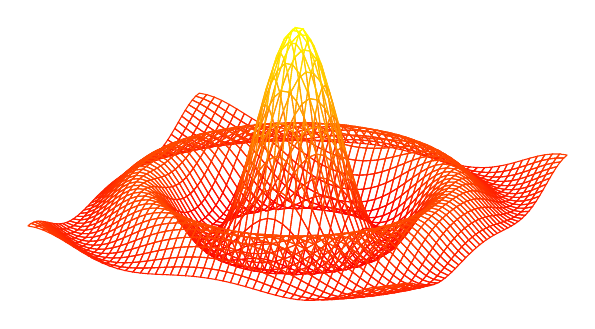
\begin{tikzpicture}
    \begin{axis}[hide axis,colormap/redyellow]
      \addplot3[mesh,samples=50,domain=-10:10]
        {5*sin(deg(sqrt(x^2+y^2)))/sqrt(x^2+y^2)};
    \end{axis}
  \end{tikzpicture}
\end{document}
